%-------------------------------------------------------------------------------
%-------------------------------------------------------------------------------
%-------------------------------------------------------------------------------
\chapter{Intégration I : point milieu}
%-------------------------------------------------------------------------------
%-------------------------------------------------------------------------------
\thispagestyle{empty}
{\sf Ce T.P. a pour but d'étudier l'erreur commise lors du calcul d'une valeur approchée d'une intégrale. On y comparera les sommes de Riemann (à gauche) avec une méthode qui n'a peut être pas été vue en cours. La démarche se généralise à toutes les méthodes, en particulier la méthode du point milieu a une efficacité semblable à la méthode du trapèze. 
Nous utiliserons les fonctions mathématiques du module \type{math}.
%--------------------------------------------------------------------------
\begin{lstlisting}
from math import *
\end{lstlisting}
%--------------------------------------------------------------------------
}
%-------------------------------------------------------------------------------
\section{Définition}
%-------------------------------------------------------------------------------
%-------------------------------------------------------------------------------
Les méthodes de calcul d'une intégrale $\displaystyle \int_a^b f(t) \d t$ consistent à découper l'intervalle $[a;b]$ en $n$ intervalles $[x_{k}; x_{k+1}]$, $0\le k < n$ avec $ x_k = a + k\frac{b-a}n$ pour $0\le k\le n$ puis à approcher l'intégrale $\displaystyle \int_{x_k}^{x_{k+1}} f(t) \text{d}t$ par une expression simple :
%-------------------------------------------------------------------------------
\begin{enumerate}
    \item $(x_{k+1} -x_k)f(x_k)$ pour la méthode des rectangles à gauche,
    \item $(x_{k+1} -x_k)f(x_{k+1})$ pour la méthode des rectangles à droite,
    \item $\displaystyle (x_{k+1} -x_k)\frac{f(x_k)+f(x_{k+1})}2$ pour la méthode des trapèzes
\end{enumerate}
%-------------------------------------------------------------------------------

Voici une écriture du calcul avec la méthode des rectangles à gauche :
%--------------------------------------------------------------------------
\begin{lstlisting}
def rect_g(f, a, b, n):
    pas = (b-a)/n
    s = 0
    for k in range(n):
        c = a + k*pas
        s = s + f(c)
    return s*pas
\end{lstlisting}
%--------------------------------------------------------------------------
\newpage
Nous allons implémenter ici une autre méthode, nommée "du point milieu" :
\[\int_{x_k}^{x_{k+1}} f(t) \text{d}t\simeq (x_{k+1} -x_k)f\left(\frac{x_k + x_{k+1}}2\right)\]
%--------------------------------------------------------------------------
%--------------------------------------------------------------------------
\begin{Exercise}[title ={Écriture}]\it
Écrire la fonction \type{point\_m(f, a, b, n)} qui approche l'intégrale de $f$ entre $a$ et $b$ par cette méthode en subdivisant $[a;b]$ en $n$ intervalles.
\end{Exercise}
%--------------------------------------------------------------------------
\begin{Answer}
\begin{lstlisting}
def point_m(f, a, b, n):
    pas = (b-a)/n
    s = 0
    for k in range(n):
        c = a + (k + 1/2)*pas
        s = s + f(c)
    return s*pas
\end{lstlisting}
\end{Answer}
%--------------------------------------------------------------------------
%-------------------------------------------------------------------------------
\section{Calculs approchés de $\pi$}
%-------------------------------------------------------------------------------
Nous allons approcher la valeur de $\displaystyle I = \int_0^1 \frac 4{1+t^2} dt=\pi$.
%--------------------------------------------------------------------------
%--------------------------------------------------------------------------
\begin{Exercise}\it
Créer la fonction $f_1$ : $\displaystyle t \mapsto \frac 4{1+t^2}$
\end{Exercise}
%--------------------------------------------------------------------------
\begin{Answer}
\begin{lstlisting}
def f1(t):
    return 4/(1+t**2)
\end{lstlisting}
\end{Answer}
%--------------------------------------------------------------------------
%--------------------------------------------------------------------------
L'erreur commise pour $n$ est l'écart entre $\pi$ est la valeur calculée : 

\type{abs(rect\_g(f1, 0, 1, n) - pi)} ou \type{abs(point\_m(f1, 0, 1, n) - pi)}
%--------------------------------------------------------------------------
%--------------------------------------------------------------------------
\begin{Exercise}\it
Calculer les erreurs pour $n=10^p$ avec $p\in\{1, 2, 3, 4, 5, 6, 7\}$ (le dernier calcul peut être long) avec chacune des deux méthodes.

Que peut-on dire de cette erreur lorsque $n$ est multiplié par 10 ?
\end{Exercise}
%--------------------------------------------------------------------------
\begin{Answer}

\begin{lstlisting}
for p in range(1, 8):
    n = 10**p
    e1 = abs(rect_g(f1, 0, 1, n) - pi)
    e2 = abs(point_m(f1, 0, 1, n) - pi)
    print("Pour n = {}, l'erreur est : ".format(n))
    print("  {:7.1e} pour rect_g, {:7.1e} pour point_m".format(e1, e2))
\end{lstlisting}

\begin{lstlisting}
Pour n = 10, l'erreur est : 
  9.8e-02 pour rect_g, 8.3e-04 pour point_m
Pour n = 100, l'erreur est : 
  1.0e-02 pour rect_g, 8.3e-06 pour point_m
Pour n = 1000, l'erreur est : 
  1.0e-03 pour rect_g, 8.3e-08 pour point_m
Pour n = 10000, l'erreur est : 
  1.0e-04 pour rect_g, 8.3e-10 pour point_m
Pour n = 100000, l'erreur est : 
  1.0e-05 pour rect_g, 8.4e-12 pour point_m
Pour n = 1000000, l'erreur est : 
  1.0e-06 pour rect_g, 2.9e-14 pour point_m
Pour n = 10000000, l'erreur est : 
  1.0e-07 pour rect_g, 6.2e-14 pour point_m
\end{lstlisting}

Pour les premières valeurs de $n$, l'erreur est divisée par 10 (resp. par 100) chaque fois que $n$ est multiplié par 10 pour la méthode des rectangles (resp. du point milieu).

Dans le cas du point milieu, il n'y a plus d'amélioration à la fin.
\end{Answer}
%--------------------------------------------------------------------------
%--------------------------------------------------------------------------
\section{Erreur comme fonction de $n$}
%-------------------------------------------------------------------------------
%-------------------------------------------------------------------------------

On souhaite maintenant étudier plus précisément  l'erreur en fonction de $n$.
%--------------------------------------------------------------------------
%--------------------------------------------------------------------------
\begin{Exercise}\it
Définir une liste d'entiers \type{N} prenant 100 valeurs de 5000 à 500000 espacées de 5000 :

\type{N = [5000, 10000, 15000, ..., 495000, 500000]}

Définir la liste \type{err\_g} correspondant aux erreurs de la méthode des rectangles pour le calcul de $I$.

Définir la liste \type{err\_m} correspondant aux erreurs de la méthode du point milieu pour le calcul de $I$.

Le calcul peut être un peu long (10 secondes).
\end{Exercise}
%--------------------------------------------------------------------------
\begin{Answer}
\begin{lstlisting}
taille = 100 
pas = 5000
N  = [0]*taille
err_g = [0]*taille
err_m = [0]*taille
for i in range(taille):
    N[i] = (i+1)*pas
    err_g[i] = abs(pi -  rect_g(f1, 0, 1, N[i]))
    err_m[i] = abs(pi -  point_m(f1, 0, 1, N[i]))
\end{lstlisting}

On peut utiliser les sucres syntactiques de Python :
\begin{lstlisting}
taille = 100 
pas = 5000
N  = [(i+1)*pas for i in range(taille)]
err_g = [abs(pi - rect_g(f1, 0, 1, n)) for n in N]
err_m = [abs(pi - point_m(f1, 0, 1, n)) for n in N]
\end{lstlisting}
\end{Answer}
%--------------------------------------------------------------------------
%--------------------------------------------------------------------------
\medskip

On peut alors représenter le graphe de l'erreur en fonction de $n$.

On utilise le module \type{matplotlib}, à importer.
\begin{lstlisting}
import matplotlib.pyplot as plt
\end{lstlisting}

\type{plt.plot(X, Y)} calcule le graphe, ce sont les segments de droite joignant les points de coordonnées \type{(X[i], Y[i])} et \type{(X[i+1], Y[i+1])}. La fonction demande deux listes de même taille\footnote{\type{plt.plot(Y)} est possible, l'abscisse est alors déterminée par l'indice.}. \type{plt.show()} dessine alors le graphe à l'écran.
%--------------------------------------------------------------------------
\begin{lstlisting}
plt.plot(N, err_g, label = "Rectangles")
plt.plot(N, err_m, label = "Point milieu")
plt.legend()
plt.show()
\end{lstlisting}
%--------------------------------------------------------------------------
Ici on peut conjecturer que l'erreur est de la forme $e = \frac K{n^p}$. Pour le mettre en évidence on remarque que $\ln(e) = \ln(K) - p \ln(n)$ ; une échelle logarithmique devrait donner une droite de pente $-p$.

On impose une échelle logarithmique avec les instruction 
\type{plt.xscale('log')} et \type{plt.yscale('log')}
%--------------------------------------------------------------------------
\begin{lstlisting}
plt.xscale('log')
plt.yscale('log')
plt.plot(N, err_g, label = "Rectangles")
plt.plot(N, err_m, label = "Point milieu")
plt.legend()
plt.show()
\end{lstlisting}
%--------------------------------------------------------------------------
\begin{center}
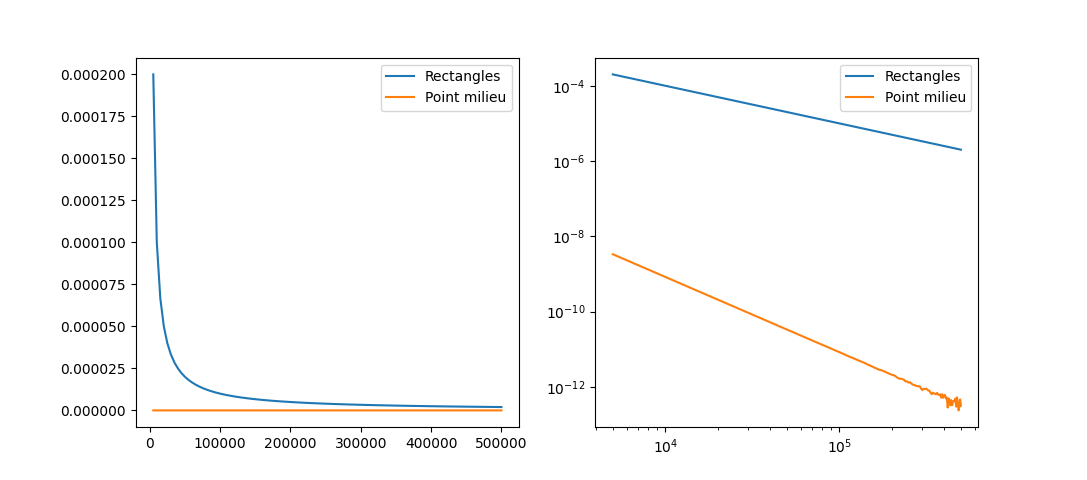
\includegraphics[scale=0.5]{TP/Images/TP18_err_lin_log.png}
\end{center}
%--------------------------------------------------------------------------
%--------------------------------------------------------------------------
\begin{Exercise}\it
À quoi sont dues les variations pour les grandes valeurs de $n$ dans le cas du point milieu ?
\end{Exercise}
%--------------------------------------------------------------------------
\begin{Answer}

On fait une somme de  $10^5$ termes, chacun étant approché avec une précision de $10^{-17}$ ; on aboutit à une erreur de l'ordre de $10^{-12}$ qui est l'approximation mathématique. On ne pourra plus améliorer la précision.
\end{Answer}
%--------------------------------------------------------------------------
%--------------------------------------------------------------------------
On peut conjecturer que la pente est $-1$, l'erreur serait de la forme $\displaystyle \frac{K_1}{n}$ pour la méthode des rectangles et une pente $-2$ avec une erreur de la forme $\displaystyle \frac{K_2}{n^2}$ pour la méthode du point milieu.

Pour le vérifier, on peut calculer la liste des erreurs multipliées par $n^p$.
%--------------------------------------------------------------------------
%--------------------------------------------------------------------------
\begin{Exercise}\it
Calculer et représenter les listes \type{K\_g} et \type{K\_m} telles que 

\type{K\_g[i] = err\_g[i]*N[i]} et \type{K\_m[i] = err\_m[i]*N[i]**2}.
\end{Exercise}
%--------------------------------------------------------------------------
\begin{Answer}
\begin{lstlisting}
n = len(N)
K_g = [0]*n
K_m = [0]*n
for i in range(n):
    K_g[i] = err_g[i]*N[i]
    K_m[i] = err_m[i]*N[i]**2
    
plt.plot(N, K_g, label = "Rectangles")
plt.plot(N, K_m, label = "point milieu")
plt.legend()
plt.show()
\end{lstlisting}
%--------------------------------------------------------------------------
\begin{center}
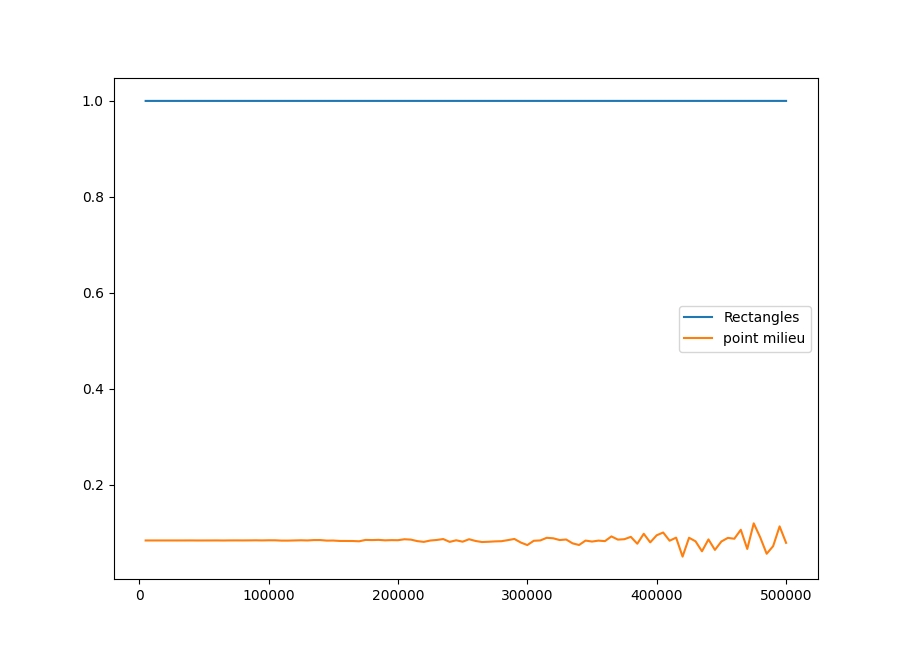
\includegraphics[scale=0.5]{TP/Images/TP18_err_K.png}
\end{center}
\end{Answer}
%--------------------------------------------------------------------------
%--------------------------------------------------------------------------
\section{Un résultat contre-intuitif}
%-------------------------------------------------------------------------------
%-------------------------------------------------------------------------------
Dans cette partie on ne suppose plus que la fonction à intégrer est donnée sous forme d'une évaluation en tout point par une fonction Python mais qu'elle n'est connue que par ses valeurs en $N$ points, on dit qu'elle est tabulée. Ce sera souvent le cas pour des fonctions calculées expérimentalement : un processus d'acquisition a enregistré les valeurs selon une période donnée.
%--------------------------------------------------------------------------
%--------------------------------------------------------------------------
\begin{Exercise}\it
Écrire les instructions qui permettent de calculer la liste \type{F1} des valeurs des $f_1(t_k)$ pour $t_k = k.10^{-3}$, $0 \le k \le 1000$ ; \type{F1} sera de longueur 1001.

On calculera aussi la liste \type{T} des $t_k$.
\end{Exercise}
%--------------------------------------------------------------------------
\begin{Answer}
\begin{lstlisting}
N1 = 1001
T = [0]*N1
F1 = [0]*N1
for k in range(N1):
    T[k] = k/(N1 - 1)
    F1[k] = f1(T[k])
\end{lstlisting}
\end{Answer}
%--------------------------------------------------------------------------
%--------------------------------------------------------------------------
Ces listes permettent de tracer le graphe de $f_1$ : \type{plt.plot(T, F1)}.
%--------------------------------------------------------------------------
\begin{center}
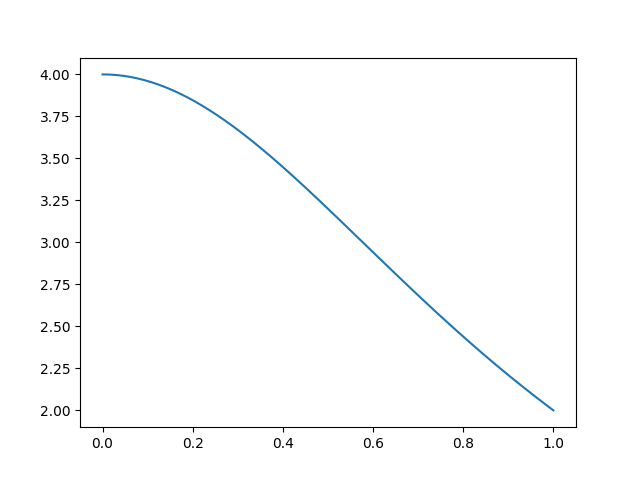
\includegraphics[scale=0.5]{TP/Images/TP18_f1.png}
\end{center}
%--------------------------------------------------------------------------
Le calcul d'une valeur approchée de l'intégrale est maintenant unique pour chaque méthode.

Si $T=[t_0, t_1, \ldots, t_{n-1}]$ est la liste des abscisses et si $Y=[y_0, y_1, \ldots, y_{n-1}]$ est la liste des ordonnées avec $F(t_k) = y_k$ alors, pour la méthode des rectangles à gauche,

\[\int_{t_0}^{t_{n-1}}f(t)\text{d}t \simeq \sum_{k=0}^{n-2}f(t_k)(t_{k+1} - t_k)=(t_1-t_0)\sum_{k=0}^{n-2}y_k\]

Ici on a supposé que le pas $t_{k+1} - t_k$ était constant, ce qui sera vrai.
%--------------------------------------------------------------------------
%--------------------------------------------------------------------------
\begin{Exercise}\it
Écrire une fonction \type{integrale\_rg(T, Y)} qui calcule l'intégrale de la fonction représentée par \type{Y} sur $[a; b]$ où $a$ et $b$ sont les valeurs extrêmes de la liste \type{T} supposée à pas constant.

Quel est l'erreur commise pour le calcul de $I$ ?
\end{Exercise}
%--------------------------------------------------------------------------
\begin{Answer}
\begin{lstlisting}
def integrale_rg(T, Y):
    s = 0
    n = len(T)
    pas = T[1] - T[0]
    for k in range(n-1):
        s = s + Y[k]
    return s*pas
    
print(abs(pi - integrale_rg(T, F1)))
\end{lstlisting}

L'erreur de de l'ordre de $10^{-3}$.
\end{Answer}
%--------------------------------------------------------------------------
%--------------------------------------------------------------------------
Dans le cas de la méthode du point milieu, comme on a besoin de la valeur de $f$ au milieu de l'intervalle, on va découper l'intégrale en somme de termes de la forme $\displaystyle \int_{t_{2k}}^{t_{2(k+1)}}f(t)\text{d}t$ que l'on approche par $f(t_{2k+1})(t_{2(k+1)} - t_{2k})=f(t_{2k+1})(t_2 - t_0)$. 

On ne peut utiliser cette méthode que si la {\bf longueur est impaire}.
%--------------------------------------------------------------------------
%--------------------------------------------------------------------------
\begin{Exercise}\it
Écrire une fonction \type{integrale\_pm(T, Y)} qui calcule l'intégrale de la fonction représentée par \type{Y} sur $[a; b]$ où $a$ et $b$ sont les valeurs extrêmes de la liste \type{T} supposée à pas constant et de longueur impaire. On emploiera la méthode du point milieu.

Quel est l'erreur commise pour le calcul de $I$ ?

\end{Exercise}
%--------------------------------------------------------------------------
\begin{Answer}
\begin{lstlisting}
def integrale_pm(T, Y):
    s = 0
    n = len(T)
    pas = T[2] - T[0]
    for k in range(1, n, 2):
        s = s + Y[k]
    return s*pas

print(abs(pi - integrale_pm(T, F1)))
\end{lstlisting}

L'erreur de de l'ordre de $4.10^{-7}$.
\end{Answer}
%--------------------------------------------------------------------------
%--------------------------------------------------------------------------
On aboutit à un résultat paradoxal : on obtient une bien meilleure approximation en employant seulement la moitié des points !
%--------------------------------------------------------------------------
%--------------------------------------------------------------------------
\subsection{Complément}
%-------------------------------------------------------------------------------
%-------------------------------------------------------------------------------
En général on emploie plutôt la méthode des trapèzes qui donne un résultat un peu meilleur que le point milieu.
%--------------------------------------------------------------------------
%--------------------------------------------------------------------------
\begin{Exercise}\it

Écrire une fonction \type{integrale\_tr(T, Y)} qui calcule l'intégrale de la fonction représentée par \type{Y} sur $[a; b]$ où $a$ et $b$ sont les valeurs extrêmes de la liste \type{T} supposée à pas constant avec la méthode des trapèzes.

Quel est l'erreur commise pour le calcul de $I$ ?

\end{Exercise}
%--------------------------------------------------------------------------
\begin{Answer}
\begin{lstlisting}
def integrale_tr(T, Y):
    s = (Y[-1] - Y[0])/2
    n = len(T)
    pas = T[1] - T[0]
    for k in range(n-1):
        s = s + Y[k]
    return s*pas

print(abs(pi - integrale_tr(T, F1)))
\end{lstlisting}


L'erreur de de l'ordre de $2.10^{-7}$.
\end{Answer}
%--------------------------------------------------------------------------
%--------------------------------------------------------------------------




